\section{Results}
\label{sec:results}

\subsection{Performance}

\begin{itemize}
	\item How long does it take to do matrix calculation for one consensus?
\end{itemize}

\subsection{Churn rate analysis}
Narrow distribution, with 99.9\% of all churn values being in the interval $[0, 0.07624282]$.

\begin{table}[ht]
	\centering
	\begin{tabular}{llllll}
	Min. & 1st Qu. & Median & Mean & 3rd Qu. & Max. \\
	\hline
	0.00423 & 0.01782 & 0.02647 & 0.02930 & 0.03972 & 0.54500 \\
	\end{tabular}
	\caption{Summary of churn rate distribution.}
	\label{tab:churn_distribution}
\end{table}

\begin{figure}[t]
	\centering
	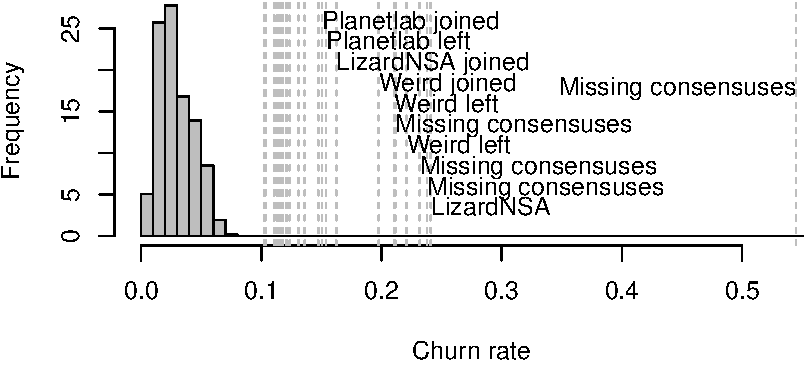
\includegraphics[width=0.49\textwidth]{diagrams/churn.pdf}
	\caption{Histogram of the churn rates between all 67,671 consensuses.  21
		outliers in the interval $[0.1, 0.15[$ are marked, and 11 outliers in
		the interval $[0.15, 0.54499]$ are also labelled.}
	\label{fig:churn}
\end{figure}

\subsection{Fingerprint anomalies}

\begin{figure}[t]
	\centering
	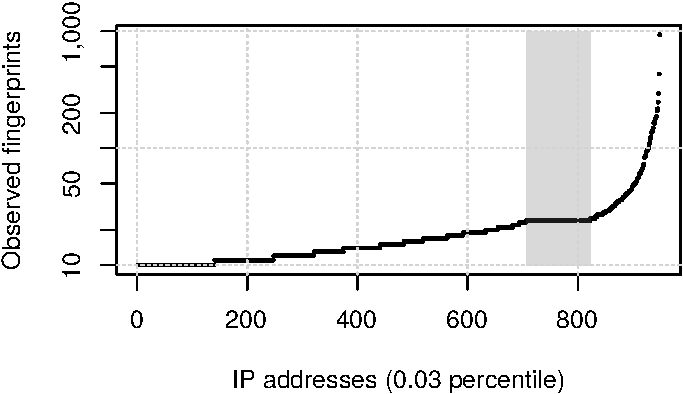
\includegraphics[width=0.49\textwidth]{diagrams/fingerprints.pdf}
	\caption{Foo.}
	\label{fig:fingerprints}
\end{figure}

There is an interesting plateau at 24, encompassing xx relays.

\subsection{Sybil groups}
\label{sec:sybil_groups}
Table~\ref{tab:sybils} contains all the Sybil groups we identified.  For every
group, we document when it first appeared in the Tor network, its ``name,''
size, and a description of its characteristics.

\begin{table*}[t]
\centering
\begin{tabular}{l c c p{10cm}}
\textbf{First seen} & \textbf{Group ID} & \textbf{\# of relays} & \textbf{Characteristics} \\
\hline
2015-07-10 & denkonet & 58 & Unknown. \\
2015-07-02 & cloudvps & 55 & Unknown. \\
2015-06-29 & onion rewrite & 55 & Transparent onion URL rewriting. \\
2015-06-17 & 1jabberat & X & not good. \\
2015-06-05 & hsdirscanner2 & 105 & Scanning HSDirs. \\
2015-06-03 & abcd & 28 & Changing fingerprints. \\
2015-05-29 & facebook hsdirs & 6 & Became HSDirs responsible for facebook.  \\
2015-05-20 & hsdirscanner1 & 102 & Scanning HSDirs. \\
2015-04-22 & sigaint & 83 & Targeting (at least) sigaint.org. \\
2015-03-11 & bitcoin-redirect & 24 & Attacking Bitcoin sites by redirecting to own web server. \\
2015-XX-YY & default & many & Likely a Windows-powered botnet.  The group
features wide, geographical distribution, which is uncommon for typical Tor
relays. \\
2013-02-03 & AmazonEC2 & XX & Changed their fingerprint exactly 24 times. \\
LizardNSA & X & & Y \\
\end{tabular}
\caption{Sybil groups identified by our system.}
\label{tab:sybils}
\end{table*}

\subsection{Other anomalies}
\begin{itemize}
	\item Some events with unexpectedly high network churn.  Generally, churn
		is not problematic.  It can be problematic, however, for guard relays,
		if they change their IP addresses.

	\item Several relays changed their fingerprint an unusually high amount of
		times.  Cause often misconfiguration, but in some cases likely attacks
		on Tor's DHT.
\end{itemize}
